\section{Introduction}






Pre-training large language models (LLMs) typically involves following a learning rate schedule that decreases over a pre-determined number of steps, such as a cosine schedule \citep{loshchilov2017sgdr,touvron2023llama}, where the learning rate starts high and gradually decreases in a smooth curve following the shape of a cosine function. 
This inflexible approach makes it difficult to adapt to additional compute or data, as the learning rate schedule for all the data is not a natural continuation of the schedule used with past data. Additionally, fitting scaling laws is costly because each compute budget requires retraining to adjust the learning rate schedule \citep{hoffmann2022training}.

In contrast to the cosine learning rate, recent work~\cite{hu2024minicpm} introduces the warmup-stable-decay ($\wsd$) schedule, which does not require committing to a pre-specified total compute budget.
After a standard warm-up period, the $\wsd$ schedule maintains a main ``branch'' using  a constant learning rate indefinitely and branch off using a fast-decaying learning rate schedule to obtain intermediate checkpoints (see the second row of Figure~\ref{fig:learningrate}). Using the $\wsd$ schedule, one can continue training from a checkpoint in the main branch by resuming with the same constant learning rate and can obtain training losses for multiple compute budgets with a single run.

Empirically, the $\wsd$ schedule produces a non-traditional loss curve (see~\Cref{fig:losscurve}): during the constant learning rate phase, the loss remains higher than the loss using other schedules like the cosine schedule; but during the decay phase, it drops sharply, often leading to a better final performance compared to the cosine schedule. This raises the main question the paper aims to address: 

\begin{wrapfigure}{r}{0.4\textwidth}
    \centering
    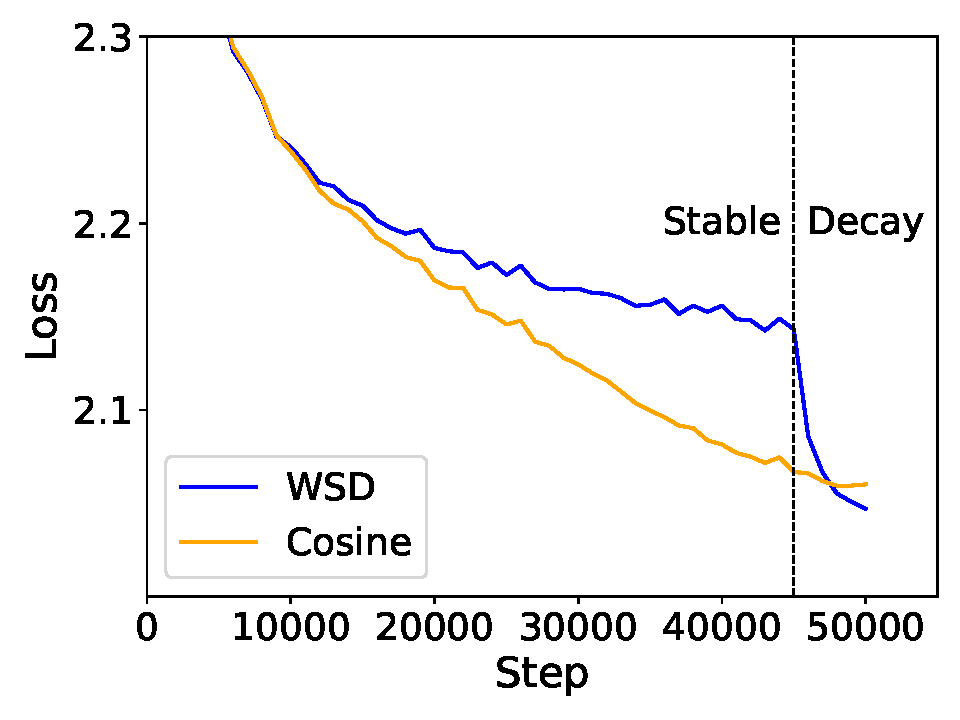
\includegraphics[width=0.4\textwidth]{figures/arxiv/loss.pdf}
    \caption{\textbf{The Distinctive Loss Curve produced by $\wsd$.} 
A constant learning rate phase, characterized by slow loss improvements, eventually leads to better validation loss after learning rate decay.}
    \label{fig:losscurve}
    \vspace{-0.3in}
\end{wrapfigure}

\emph{Why does $\wsd$ work, especially with such a non-traditional loss curve? Specifically, why does a constant learning rate phase, characterized by slow loss improvements, eventually lead to superior performance?}


\begin{figure}[t]
    \centering
    \begin{subfigure}[b]{0.36\textwidth}
        \centering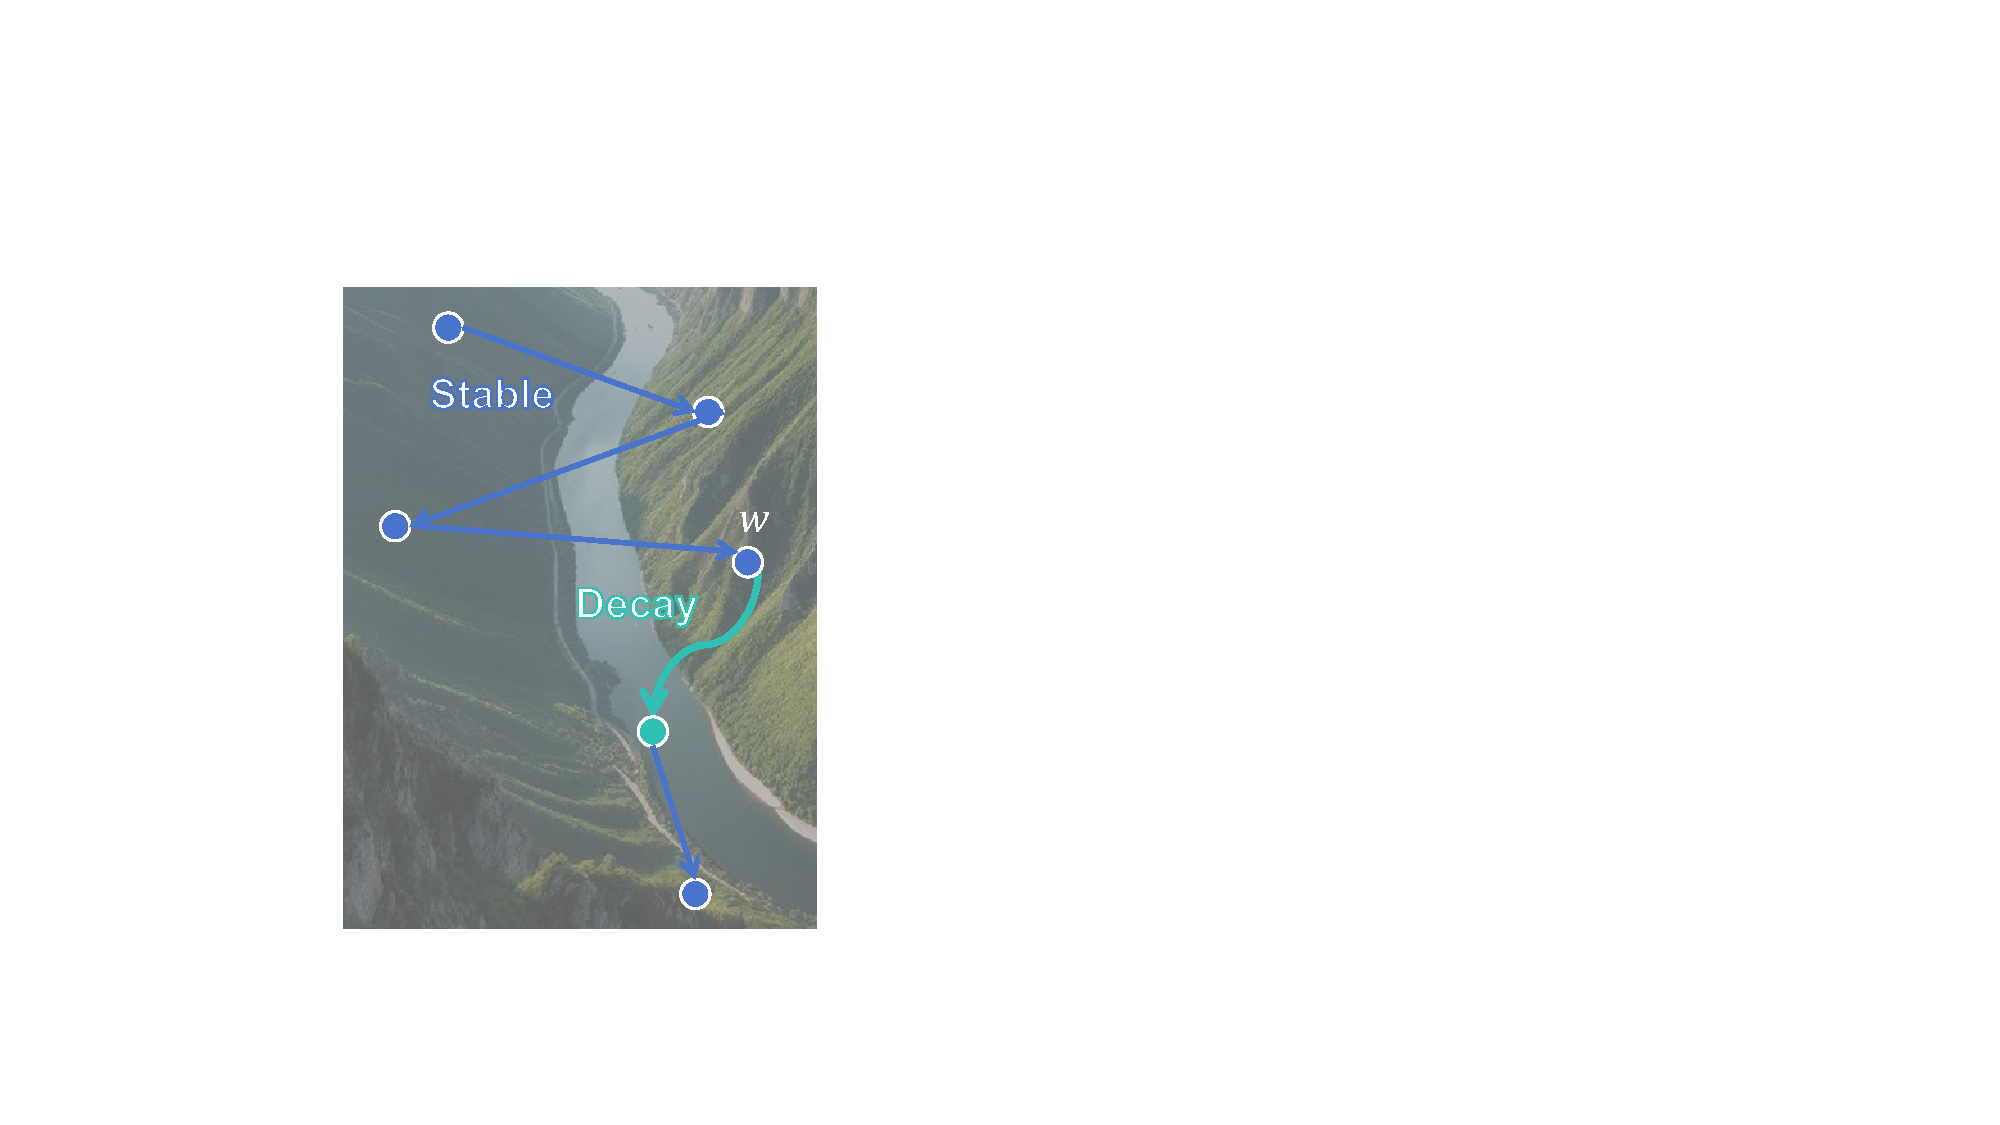
\includegraphics[width=\textwidth]{figures/arxiv/motivation_new_3.pdf}
        \caption{River Valley Landscape}
        \label{fig:landscape}
    \end{subfigure}
    \hfill
    \begin{subfigure}[b]{0.62\textwidth}
        \centering
        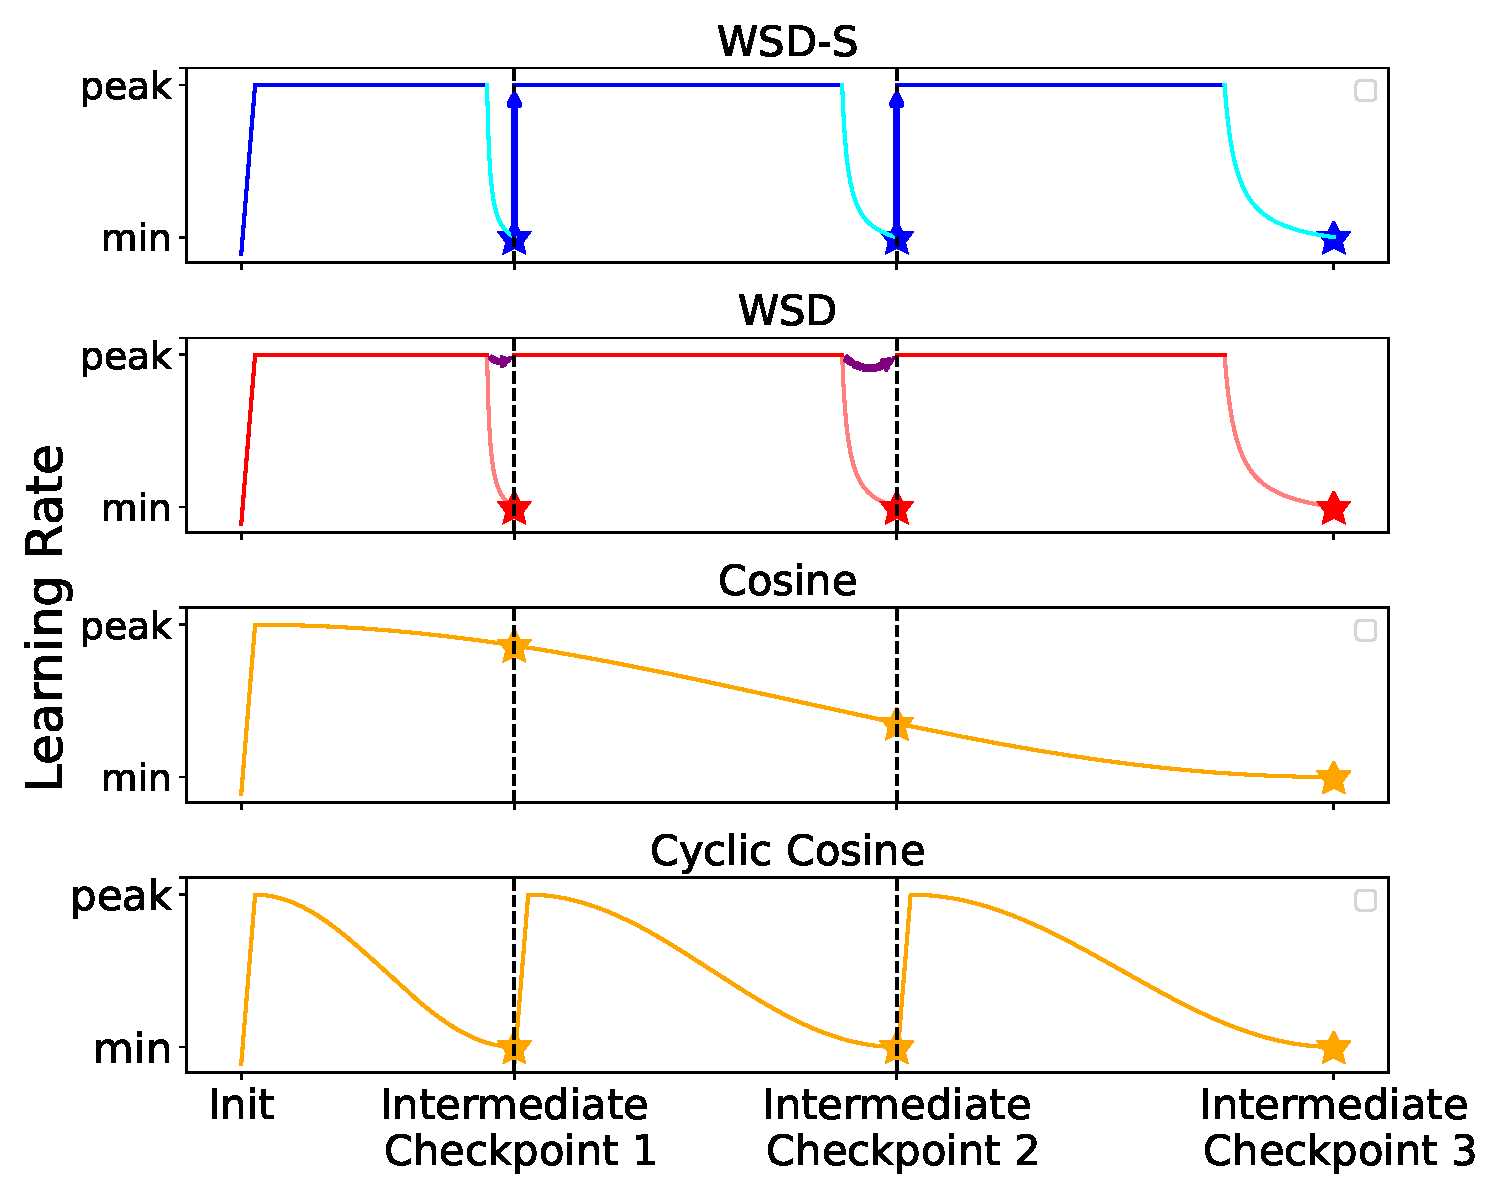
\includegraphics[width=\textwidth]{figures/arxiv/schedule_new.pdf}
        \caption{Learning rate schedules}
        \label{fig:learningrate}
    \end{subfigure}
    \caption{
        We theoretically analyze the Warmup-Stable-Decay ($\wsd$) schedule and demonstrate a \textbf{river valley} loss lanscape model to explain its effectiveness (demonstrated in~\Cref{fig:landscape}). The stable phase adopts a large learning rate and the iterate will progress along the river while oscillating between the sharp hillsides. Due to the large oscillation caused by the large learning rate, the run will potentially show a higher loss compared to a run using smaller learning rate in this phase. During the decay phase, the learning rate is dropped rapidly to ease the oscillation of the iterates, driving it closer to the river, revealing the optimization progress.
        Based on our theory, we propose $\wsds$implified ($\wsds$), an effective simplification of the $\wsd$ schedule in continual learning, where we start directly using a high learning rate from previous intermediate checkpoints. We visualize the learning rate schedule in~\Cref{fig:learningrate}.
        The {\color{mypurple}{arrow}} in the second row of~\Cref{fig:learningrate} indicates $\wsd$ reinitializes the checkpoint from the last checkpoint from the constant learning rate phase instead. 
    }
    \vspace{-0.2in}
    \label{fig:mot}
\end{figure}


The first contribution of this paper is a theoretical framework to explain the underlying mechanism of $\wsd$. We characterize a type of loss landscape, called {the} river valley landscape (\Cref{def:river-valley}), and theoretically show that $\wsd$ has superior performance on such loss landscapes. 
We show that the river valley landscape can provide multiple theoretical prediction matching the empirical observations and hence can serve as a useful conceptual picture for understanding the pretraining optimization process.


As the name suggests, a river valley landscape intuitively features steeply sloping hillsides with a river winding through the bottom of the gorge (see \Cref{fig:landscape}). During the stochastic gradient-based optimization process, the iterate bounces between the hillsides as it slowly and implicitly progresses along the river direction. The loss in this landscape can be decomposed into two components: the \emph{river component}, which represents the primary loss along the river at the bottom of the hills, and the \emph{hill component}, which accounts for the additional loss caused by deviations in height from the river's course. Progress is determined primarily by the river component in the long run.
We demonstrate that when the loss function exhibits this type of landscape, a learning rate schedule should satisfy the following two key properties to effectively minimize the loss.
\vspace{-0.1in}
\begin{enumerate}[leftmargin=*]
\setlength{\itemsep}{0pt}
    \item \textbf{Sustained high learning rate.} It is advantageous to maintain a large learning rate for as long as possible during training, even at the cost of less reduction in the loss. A large learning rate yields larger  bouncing due to the stochasticity of the gradient, increasing the hill component of the loss, but it also makes faster progress in the river direction. In contrast, a small learning rate results in less bouncing, keeping the iterate close to the river, but progress along the river direction is slower. Therefore, a larger learning rate leads to faster fundamental progress minimizing the river component, which is obscured by the oscillation in the hill component. This progress will be revealed by the decay phase discussed below.
    \item \textbf{Final low learning rate.} As training nears completion, it becomes essential to reduce the learning rate. This decay minimizes the oscillations in the mountain direction to decrease the hill component and ensures that the iterates converge to a point close to the river, which has a lower loss than any nearby points up the mountain.
\end{enumerate}
\vspace{-0.1in}
In Section~\ref{sec:optimization}, we provide formal theoretical statements analyzing the trajectories of (stochastic) gradient descent on the river valley landscape, fleshing out the intuitions above. 
Among our synthetic and real-world studies supporting the river valley landscape hypothesis, an intriguing observation in language model pretraining is that the loss on the linear interpolation of two checkpoints in the stable phase exhibits a convex and unimodal shape, resembling a valley, whereas between two checkpoints in the decay phase, the loss shows a smooth monotone decay.

All the theoretical results above assume a river valley landscape. How likely does the next-token prediction loss follow this pattern, and why?
We hypothesize the river valley landscape can naturally arise from the heterogeneity in the stochasticity of different tokens: highly deterministic tokens (which often involve facts and knowledge) contribute to the "river" direction, while uncertain tokens (which often involve flexibility and ambiguity in the language) create the steep hillsides. We demonstrate this insight by showing in~\Cref{sec:data} that under a bigram toy model, indeed the loss has a river valley landscape, and empirically, most properties of the loss curves under various learning rates on the real datasets are still seen in this toy model. We further show that the stable learning rate phase learns the deterministic tokens whereas the decay phase learns better the stochastic tokens. 





Finally, we discuss the limitations of $\wsd$ within our framework and how to go beyond it. In $\wsd$, once an intermediate checkpoint is reached, the model and optimizer are rolled back to the end of the stable phase before resuming training with a constant learning rate. However, our theory suggests that the decay phase also contributes to progress along the river direction, so discarding this part of the progress is unnecessary. Moreover, when an organization pretrains an LLM with $\wsd$, it needs to release the last checkpoint in a stable-phase to facilitate continual pretraining for another party, adding extra complexity.

To overcome this limitation, we propose a simplified and improved version of $\wsd$, called \textbf{$\wsds$}, for continual learning. Specifically, $\wsds$ resumes training immediately from the intermediate checkpoint using a high constant learning rate, avoiding the need to roll back to a previous checkpoint.

We evaluate the effectiveness of $\wsds$ with extensive experiments on LLMs from 0.1B to 1.2B parameters in a continual learning setting with 50B, 100B, and 200B tokens as the three target compute budgets. We empirically show that $\wsds$ has performance comparable with independent oracle runs with cosine learning rate schedules optimally tuned on each of the three budgets. Furthermore, $\wsds$ leads to a better validation loss than $\wsd$ under the same compute budgets due to the re-use of the decay period. We also show through ablation studies that the performance is relatively insensitive to the precise fraction of time spent decaying as long as it is near $10\%$ and the decay does not start shortly after a coincidental loss spike.
